\documentclass[conference]{IEEEtran}
\IEEEoverridecommandlockouts
% The preceding line is only needed to identify funding in the first footnote. If that is unneeded, please comment it out.
\usepackage{cite}
\usepackage{amsmath,amssymb,amsfonts}
\usepackage{algorithmic}
\usepackage{graphicx}
\usepackage{textcomp}
\usepackage{xcolor}
\usepackage{derivative}
\def\BibTeX{{\rm B\kern-.05em{\sc i\kern-.025em b}\kern-.08em
    T\kern-.1667em\lower.7ex\hbox{E}\kern-.125emX}}
\begin{document}

\title{Effect of Injection and Valve Timing on Combustion Characteristics and Performance of Port-Fuelled Hydrogen Internal Combustion Engines
}

\author{\IEEEauthorblockN{I.M. Wickramaarachchi}
\IEEEauthorblockA{\textit{Department of Mechanical Engineering} \\
\textit{University of Moratuwa}\\
Katubedda, Sri Lanka \\
waisurumangala@gmail.com}
\and
\IEEEauthorblockN{J.S. Rassdeen}
\IEEEauthorblockA{\textit{Department of Mechanical Engineering} \\
\textit{University of Moratuwa}\\
Katubedda, Sri Lanka \\
waisurumangala@gmail.com}
\and
\IEEEauthorblockN{S. Kalana}
\IEEEauthorblockA{\textit{Department of Mechanical Engineering} \\
\textit{University of Moratuwa}\\
Katubedda, Sri Lanka \\
waisurumangala@gmail.com}
\and
\IEEEauthorblockN{N.A.I.D. Nissanka}
\IEEEauthorblockA{\textit{Department of Mechanical Engineering} \\
\textit{University of Moratuwa}\\
Katubedda, Sri Lanka \\
waisurumangala@gmail.com}
\and
\IEEEauthorblockN{Isuru Wickramaarachchi}
\IEEEauthorblockA{\textit{Department of Mechanical Engineering} \\
\textit{University of Moratuwa}\\
Katubedda, Sri Lanka \\
waisurumangala@gmail.com}
}

\maketitle

\begin{abstract}
The urgency of mitigating global warming has propelled hydrogen to the forefront as an alternative fuel.
However, abnormal combustion events pose a significant challenge in the development of Hydrogen Internal Combustion Engines (ICEs).
Adjustments of engine design parameters have demonstrated the possibility of controlling these issues.
Particularly, valve and injection timing are critical in mixture formation—a determinant of combustion behavior and engine performance.
Although previous research has primarily focused on the isolated effects of these parameters, their interdependence on each other is highly undeniable.
In this project, numerical simulations are carried out with detailed chemistry solver to comprehensively analyze the combined effect of valve and injection timing on the combustion characteristics and performance of port-fueled Hydrogen ICEs.
\end{abstract}

\begin{IEEEkeywords}
valve timing, injection timing, performance, combustion characteristics, hydrogen
\end{IEEEkeywords}

\section{Introduction}

Global warming presents the most severe environmental challenge today, primarily driven by the increased carbon dioxide (CO2) emissions from the consumption of fossil fuels.
The transportation sector, which heavily relies on ICEs, remains a major contributor to these emissions.
Consequently, the urgency to make these engines more sustainable and environmentally friendly is undeniable.
Efforts to address this issue led to the exploration and adoption of alternative fuels.
In this regard, hydrogen has emerged as a compelling option, taking advantage of its favourable combustion characteristics together with zero carbon emissions.\\

The literature identifies two distinct types of hydrogen ICEs: Port Fuel Injection (PFI) and Direct Injection (DI) engines.
PFI involves injecting fuel into the intake manifold, where it mixes with air before reaching the combustion chamber.
In contrast, DI engines inject hydrogen directly into the chamber during the compression stroke, initiating the ignition of the compressed air-fuel mixture.
Particularly, in DI engines, the processes of fuel-air mixing, and combustion occur simultaneously, leading to less time available for mixture formation.
To achieve sufficient mixing, higher injection pressures and precisely manufactured injectors are required, which leads to increased costs.
Conversely, PFI separates the mixing and combustion processes, affording more time for the creation of a uniform fuel-air mixture, eliminating the necessity for precisely manufactured injectors and the application of high injection pressures.
Therefore, PFI hydrogen engines represent a more viable solution for the rapid adaptation of alternative fuels.\\

Abnormal combustion including knocking and backfire are major problems found in hydrogen engines.
It has been demonstrated that those can be controlled by changing various design parameters including valve timing and injection timing.
Among the other parameters, valve and injection timing heavily affect the trapped hydrogen mass and mixture formation, which defines the combustion characteristics of ICEs.
The combustion process can lead to incomplete combustion or knocking combustion depending on the formed fuel-air mixture.\\

Although valve and injection timing are separately studied, their interdependency on each other is highly undeniable.
Both these parameters collectively define the mixture and thereby combustion characteristics and performance.
Therefore, a comprehensive understanding of the combined effect of valve and injection timing on combustion characteristics and performance is necessary to control injection timing and valve timing, in Hydrogen ICEs.\\

\section{Litreture Review}

Several studies showed the effect of valve and injection timing on combustion characteristics and performance.

\subsection{Injection Timing}

Wang \cite{b1} changed injection start times and monitored the hydrogen mass within the cylinder with crank angle.
The amount of trapped mass and mass backflow was different under each scenario.
The early injection caused less amount of backflow, and a higher fraction of mass could flow into the cylinder.
The backflow of hydrogen can be seen in every case after the compression stroke starts (after 540 CAD).
It can be explained using the push generated by the upward movement of the piston.
If the hydrogen injection is delayed, more hydrogen mass would be affected by this negative push, consequently reducing trapped hydrogen mass.
Yun \cite{b2} has measured the trapped hydrogen mass considering a wider range of injection timing.
In addition to the decreasing trend of trapped mass with delayed hydrogen injection, the effect of excessively early injection was also identified.
In combination, trapped hydrogen mass first increased and then decreased with the change of injection timing.
An optimum injection timing to trap the maximum amount of hydrogen mass could be observed.
Yun \cite{b2} also showed that the variation of indicated power and thermal efficiency was highly correlated with trapped hydrogen mass.
Therefore, to achieve higher engine performance, trapped hydrogen mass should be maximized.\\

Literature gives evidence of forming locally concentrated hydrogen mass near inlet valve seats due to improper injection timing.
Duan \cite{b3} showed that local concentration first increases and then decreases with injection delay.
When the injection is too early, hydrogen enters the inlet port and spreads towards the inlet valve before the valve opens.
When the injection is too late, hydrogen injection continuous after the intake valve closes, causing a high concentration mixture.
Liu \cite{b4} also showed this increasing trend of local concentration with excessively delayed injection timing.
In addition, excessively early or delayed injection also increases the maximum pressure in the intake port, following the same trend as the local concentration.
In the intermediate injection times, the pressure rise was minimal.
Backfire as an abnormal combustion phenomenon, usually characterized by increased intake manifold pressure.
Therefore, a comparison of the local concentration of hydrogen mass and intake manifold pressure implies that the local concentration of hydrogen near valve seats can strongly influence the backfiring risk.
Consequently, local hydrogen concentration can be used to identify the backfire possibility in port-fueled hydrogen engines.\\

\subsection{Valve Timing}

Menaa \cite{b5}, showed the variation of both trapped mass and backflow mass with the change of valve timing.
When the engine speed was lower than 2000 rpm, delaying Inlet Valve Close (IVC) caused a reduction in cylinder mass.
The behavior is the opposite with engine speeds higher than 2000 rpm.
With early IVC, backflow mass was insignificant compared to cylinder mass.
However, it is significant when the IVC is retarded.
Higher backflow mass leads to high local concentration near inlet valves, increasing the possibility of backfire.\\

Park \cite{b6} showed the effect of Inlet Valve Open (IVO) timing on engine performance and efficiency at the engine speed of 2000 rpm.
Torque had a decreasing trend with retarding IVO, while the efficiency first increased before decreasing.
This increase in thermal efficiency during the first half of the IVO delay was due to the decrease in trapped mass.
Huynh \cite{b7} studied a wider range valve overlap range from 00 - 500 to evaluate engine performance and showed that brake torque reduces in both low and excessive Valve Overlap Times (VOTs).
Reduction of engine performance was much more significant with low VOTs than with high VOTs.
VOT of 300 was shown to be the optimum VOT for the engine operating conditions in the study.
The study also showed that the probability of backfire decreases with a decrease in valve overlap.
The backfire limiting equivalence ratio, increased up to 1.2 with zero valve overlap.
This idea of backfire control by reducing VOT is also mentioned by Lee \cite{b8}.
The study conducted experiments to show that IVO timing can be used to control backfire with an ultra-lean mixture.
Results revealed that with a delay of 100CA, backfire-free operation can be ensured.\\

From these studies it is clear that valve timing affects both trapped mass and local hydrogen concentrations, consequently affecting combustion characteristics and engine performance.

\subsection{Research Gap}

Trapped hydrogen mass should be maximized to increase the performance of the engine while keeping the local concentrations near inlet valve seats at a minimum level to prevent backfire risks.
Although researchers have tried individual adjustments of valve and injection timing, it is their combined effect which defines both trapped mass and local concentration.
To control these parameters to improve engine performance while mitigating abnormal combustion events, a comprehensive understanding of their combined effect is necessary.

\section{Numerical Model}
\subsection{Governing Equations}
Reactive flow is governed by mass and momentum equations, energy equations, and species transport equations.

\subsubsection{Mass and momentum equations}

    \begin{gather*}
        \pdv{\rho}{t} + \pdv{(\rho u)}{ x} = 0
    \end{gather*}

    \begin{gather*}
        \pdv{(\rho u)}{t} + \pdv{(\rho uv)}{y} = - \pdv{p}{x} + \pdv{\tau\textsubscript{xy}}{y} + S\textsubscript{x}
    \end{gather*}

Where $\rho$ is density, $t$ is time, $u$, $v$ and $w$ are velocity component in $x$, $y$, and $z$ directions respectively. 
$p$ is pressure, $\tau\textsubscript{xy}$ is stress tensor, and $S\textsubscript{x}$ is the momentum source component.\\

\subsubsection{Energy equation}

    \begin{gather*}
        \pdv{(\rho e)}{t} + \pdv{(\rho ev)}{y} = -p \pdv{v}{y} + \tau \textsubscript{xy} \pdv{u}{y} + \pdv{(k \pdv{T}{y})}{y} + \pdv{(\rho D \sum h_m \pdv{Y_m}{y})}{y} + S
    \end{gather*}

Where $e$ is specific internal energy, $k$ is conductivity, $T$ is temperature, $D$ is coefficient of mass diffusion, $h_m$ is species enthalpy, $Y_m$ is mass fraction of species $m$ and $S$ is source term which accounts for energy sources.\\

\subsubsection{Species transport equation}

    \begin{gather*}
        \pdv{\rho_m}{t} + \pdv{(\rho_m v)}{y} = \pdv{(\rho D \pdv{Y_m}{y})}{y} +  S_m
    \end{gather*}

Where $r_m$ is species density, $D$ is the mass diffusion coefficient, $Y_m$ is the mass fraction of species $m$ and $S_m$ is the source term which accounts for the chemical reactions.\\

\subsection{Combustion model}
SAGE detailed chemistry solver is used to model the combustion process and is explained below.\\
A multi-step chemical reaction can be expressed in the form of,

\begin{gather*}
    \sum v'\textsubscript{m,r} X_m \leftrightarrow \sum v''\textsubscript{m,r} X_m for  r = 1,2,...R
\end{gather*}

Where $M$ is the total number of species present in the chemical reaction mechanism, $R$ is the total number of elementary reactions, $v'\textsubscript{m,r}$ and $v''\textsubscript{r,m}$ are the stoichiometric coefficients of the reactants and products respectively, for the $m\textsuperscript{th}$ species in the $r\textsuperscript{th}$ reaction and $X_m$ is the chemical symbol of species $m$.\\

The net production rate of each species in a multi-step chemical reaction is given by,

\begin{gather*}
    \dot\omega = \sum_{m=1}^{M} v\textsubscript{m,r} 
\end{gather*}

Where, $v\textsubscript{m,r}$ is the coefficients difference and $q_r$ is the rate-of-progress variable for the $r\textsuperscript{th}$ elementary reaction and is given by,

\begin{gather*}
    q_r = k\textsubscript{fr} \prod_{m=1}^{M} [X_m]\textsuperscript{v'\textsubscript{m,r}} - k\textsubscript{rr} \prod_{m=1}^{M} [X_m]\textsuperscript{v''\textsubscript{m,r}}
\end{gather*}

Where, $k\textsubscript{$fr$}$ and $k_\textsubscript{$rr$}$ are the elementary forward and reverse rate coefficients for rth reaction, and $X_m$ is the molar concentration of species $m$.

\subsection{Model Description}
A single-cylinder spark ignition engine was selected for the present study.
The geometric and technical details of the engine are given in the table. 


\begin{table}[!ht]
    \centering
    \caption{Technical Details}
    \label{your_label_here}
    \begin{tabular}{|c|c|}
    \hline
    Header 1 & Header 2 \\
    \hline
    Bore & 92.6 mm \\
    Stroke & 86 mm \\
    Compression Ratio & 10.5 \\
    Equivalence Ratio & 0.59 \\
    Injection Duration & 155 CAD \\
    Engine Speed & 2000 RPM \\
    EVO & 2000 RPM \\
    EVC & 2000 RPM \\
    \hline
    \end{tabular}
    \end{table}



The three-dimensional CFD analysis was carried out using CONVERGE, a commercial CFD code.
The gas simulation was carried out with the Redlich-Kwong gas equation. 
The reaction mechanism for hydrogen combustion was taken from \cite{b9} which contains 5 elements, 10 species and 21 chemical reactions. 
A variable time step algorithm based on convection, diffusion and Mach CFL numbers was used. 
The pressure-velocity coupling was achieved using a modified Pressure Implicit with the Splitting of Operator (PISO) algorithm. 
Combustion equations were solved by SAGE while the transport equations were solved by the CFD solver to model combustion with detailed chemistry.
Unsteady Reynolds Averaged Navier-Stokes equations (URANS) were applied to model the flow field.
Turbulence effects were considered using the Renormalization group (RNG) $k-\epsilon$ model.\\

\section{Methodology}

The ignition process was modelled using a high-temperature energy source with two phases, arc and glow discharge between the electrodes of the spark plug.
Hydrogen injection is modelled using mass inflow boundary conditions.
Different input files consisting of valve lift profiles were used to set up valve movements at different valve overlap times.
Convection CFL number during the suction stroke was kept as 1 to accurately capture the mixture formation.
Results of two consecutive cycles were used to initialize the simulations to dampen out the effect of initial conditions.\\

Several mesh configurations with different base mesh sizes were tested for mesh sensitivity.
Considering the available computational resources, the sensitivity analysis was conducted only up to 8 mm base mesh.
Experimental data which have generated using a similar engine as our study \cite{b10} is used to validate the model.
Few combustion simulations to select suitable ranges for valve and injection timing.\\

Reducing VOT below 15\textsuperscript{0} would result in the opening of the intake valve after the suction stroke starts which leads to highly inefficient suction stroke and reduced trapped mass.
Further, backfire in hydrogen engines are highly evident when the valve overlap is higher than 45\textsuperscript{0} \cite{b7,b10}.
Therefore, a VOT range of 15\textsuperscript{0} – 45\textsuperscript{0} is selected for the analysis.
VOT of 30\textsuperscript{0} demonstrated the optimal engine performance in the study \cite{b7} and it lies in the middle of the selected VOT range of the study.
Therefore, a VOT of 30\textsuperscript{0} is first assumed to select a suitable range of injection timing for the analysis.
Relative Injection Start Time (IST) with respect to IVO is tested for combustion characteristics in 50 intervals.
3 modes of injection: early, balance and delayed were derived for every VOT, consequently leading to a simulation matrix of 21 operating conditions.
Results were analysed to identify trends in combustion characteristics and performance.

\section{Results and Discussion}
\subsection{Mesh sensitivity analysis and model validation}
In-cylinder pressure under each mesh configuration is shown in Fig 1.

\begin{figure}[htbp]
    \centerline{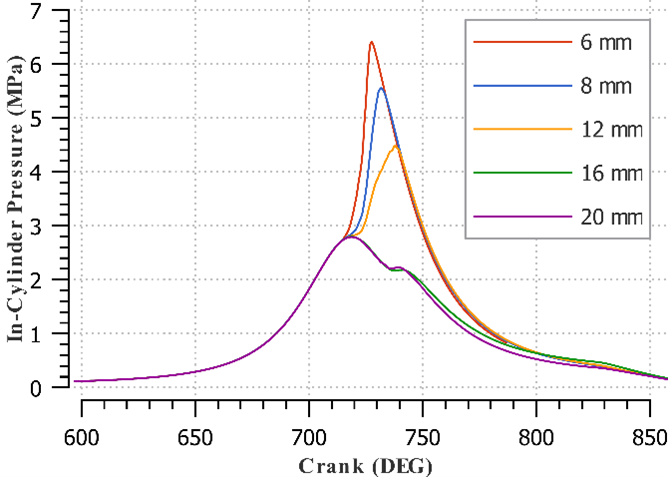
\includegraphics{plots and graphs/1.png}}
    \caption{Mesh Sensitivity}
    \label{plt_1}
    \end{figure}

The in-cylinder pressure results with the 8 mm base mesh configuration follow a similar trend to the experimental data \cite{b10}.
As \cite{b4} also mentioned simulation results can often be higher than due to limitations of the computational mesh and from the fact that only one cylinder is modelled.
However, the combustion model can be effectively utilized to find combustion characteristics and trends in engine performance.

\subsection{Range selection}
When the IST is earlier than 5\textsuperscript{0} aIVO, knocking combustion occurs.
On the other hand, when the IST is delayed more than 25\textsuperscript{0} aIVO, the mixture fails to combust properly.
Therefore, for proper combustion, injection start angles of 5\textsuperscript{0} aIVO, 15\textsuperscript{0} aIVO and 25\textsuperscript{0} aIVO were selected as early, balanced, and delayed injection.

\begin{figure}[htbp]
    \centerline{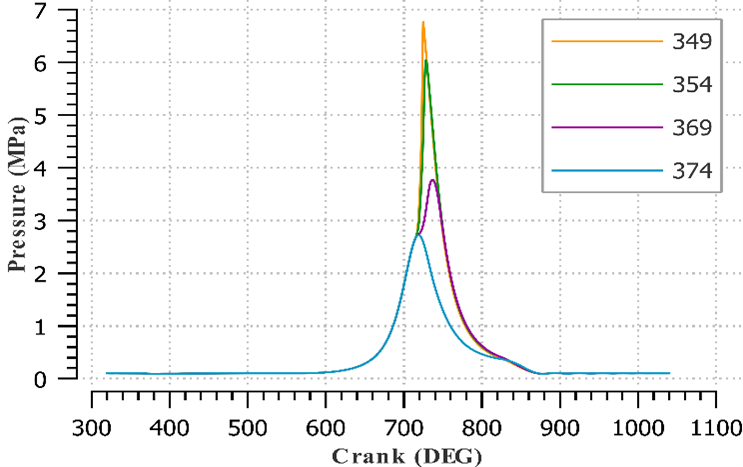
\includegraphics{plots and graphs/2.png}}
    \caption{In-cylinder Pressure at different injection modes}
    \label{plt_2}
    \end{figure}


\subsection{Trapped Mass}
When the injection is delayed with respect to IVO, for a few crack angles, only the air is flowing to the cylinder.
It leads to reduced trapped mass with injection delay.
A linear variation of trapped hydrogen mass could be observed irrespective of the injection mode.
This can be understood by observing the variation of trapped mass with the crank angle at different VOTs as shown in the figure.
When the VOT is reduced the IVC is delayed.
Therefore, a higher fraction of inlet valve open time is affected by the upward push generated by the piston during the compression stroke.
This is shown in the graph as an increased duration of mass reduction after 540\textsuperscript{0} degrees and further, increased VOT leads to an increased scavenging effect, which pushes the exhaust residual gases away from the chamber, eventually increasing the trapped mass.


\begin{figure}[htbp]
    \centerline{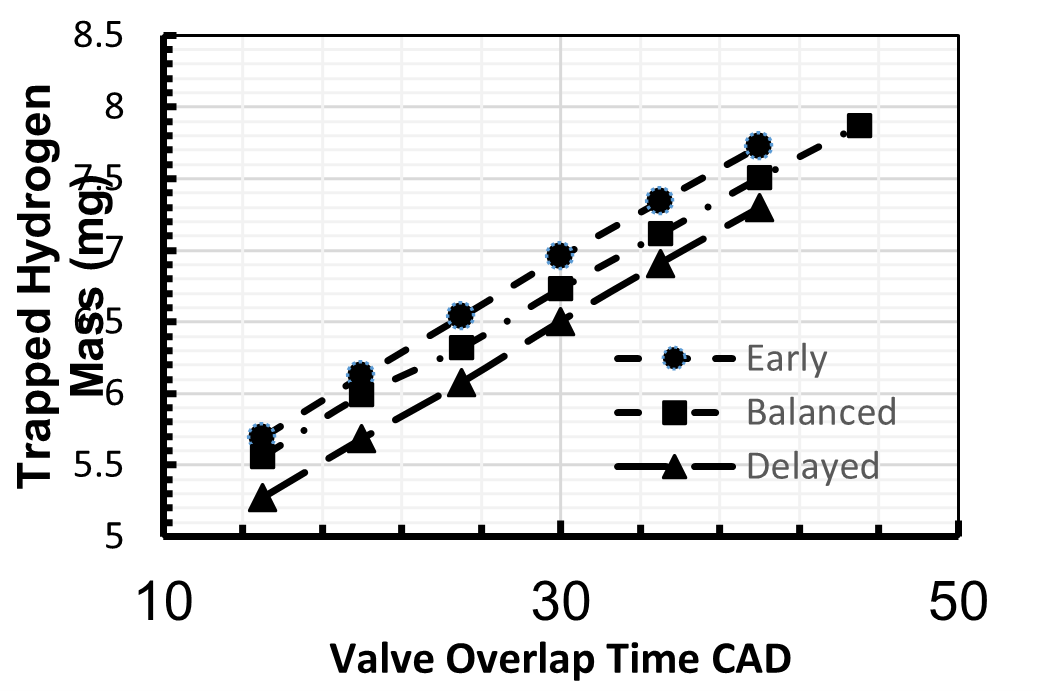
\includegraphics{plots and graphs/3.png}}
    \caption{Variation of trapped hydrogen mass at different valve times and injection modes}
    \label{plt_3}
    \end{figure}

Another important observation from the above variation is that a given trapped mass can be achieved through different parameter combinations of valve and injection timing.
Depending on the other constraints including combustion characteristics, engine performance and prevention of abnormal combustion events, controlling one parameter may be better than the other.
However, to give recommendations, further analysis is required.

\begin{figure}[htbp]
    \centerline{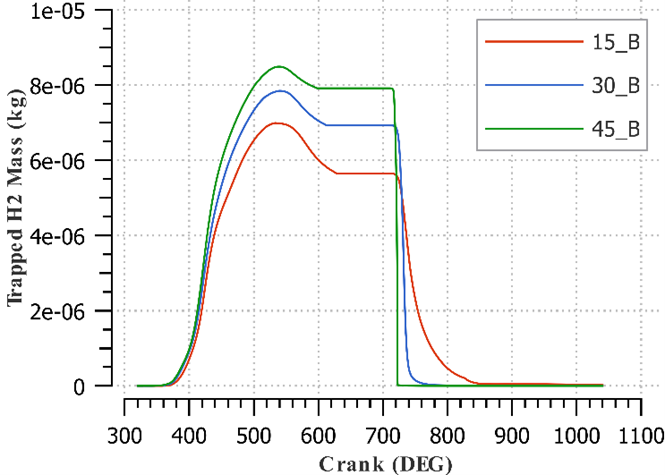
\includegraphics{plots and graphs/4.png}}
    \caption{Variation of trapped hydrogen mass at different valve times}
    \label{plt_4}
    \end{figure}

\subsection{Local concentration}
As shown in the graph, high local concentration can develop near the inlet valve during the IVO.
This localized concertation differs with different VOT and injection modes.
As shown in the graph, local hydrogen concentration near inlet valves increases with both VOT and early injection.
The ability to reduce local concentrations can only apply at reduced valve overlaps.
Valve overlap can be effectively utilized to reduce local concentrations of hydrogen during balanced and delayed injection modes.
However, the ability to reduce local concentrations by reducing VOT is insignificant with early injection mode. 
    
\begin{figure}[htbp]
    \centerline{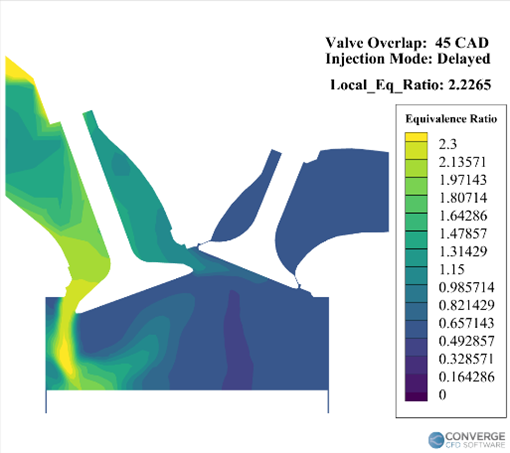
\includegraphics{plots and graphs/5.png}}
    \caption{Local concetration of hydrogen near valve seats}
    \label{plt_5}
    \end{figure}

    \begin{figure}[htbp]
        \centerline{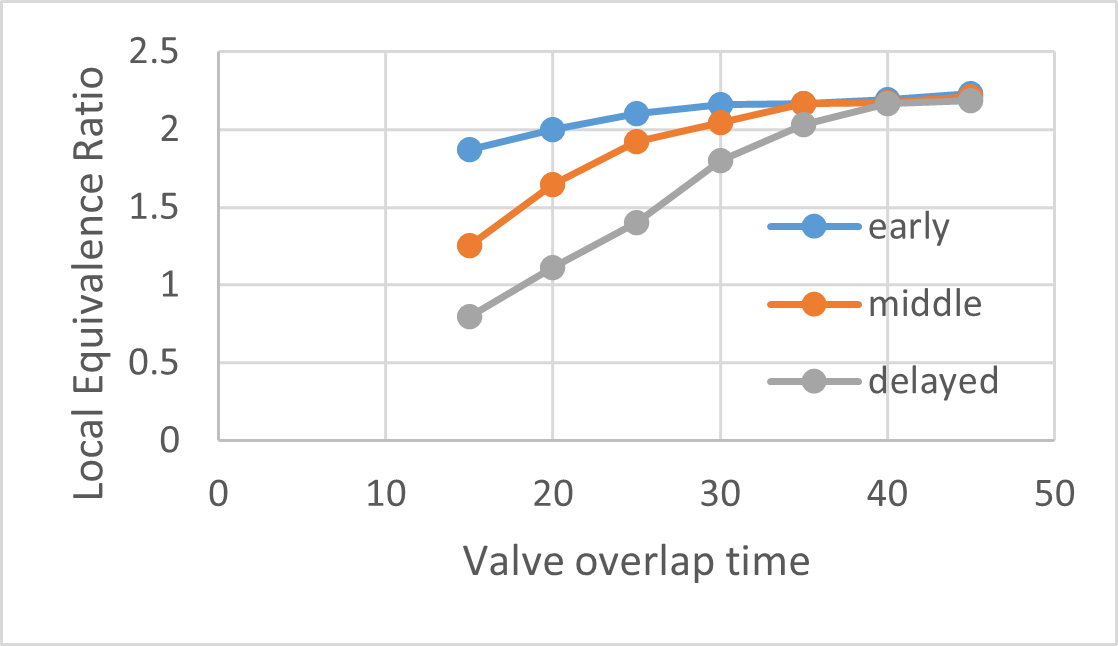
\includegraphics{plots and graphs/6.png}}
        \caption{Local concetration of hydrogen near valve seats}
        \label{plt_6}
        \end{figure}
    

\section{Conclusion}

\section{Future Works}
Effect of valve and injection timing on backfire, in particular, flame propagation.

\section*{Acknowledgment}



\begin{thebibliography}{00}
\bibitem{b1} L. Wang et al., “The effect of hydrogen injection parameters on the quality of hydrogen–air mixture formation for a PFI hydrogen internal combustion engine,” Int. J. Hydrog. Energy, vol. 42, no. 37, pp. 23832–23845, Sep. 2017, doi: 10.1016/j.ijhydene.2017.04.086.
\bibitem{b2} H. Yun, Z. Bu, Z. Yang, L. Wang, and B. Zhang, “Optimization of fuel injection timing and ignition timing of hydrogen fueled SI engine based on DOE-MPGA,” Int. J. Hydrog. Energy, vol. 48, no. 25, pp. 9462–9473, Mar. 2023, doi: 10.1016/j.ijhydene.2022.12.068.
\bibitem{b3} J. Duan, F. Liu, and B. Sun, “Backfire control and power enhancement of a hydrogen internal combustion engine,” Int. J. Hydrog. Energy, vol. 39, no. 9, pp. 4581–4589, Mar. 2014, doi: 10.1016/j.ijhydene.2013.12.175.
\bibitem{b4} X. Liu, F. Liu, L. Zhou, B. Sun, and H. Schock, “Backfire prediction in a manifold injection hydrogen internal combustion engine,” Int. J. Hydrog. Energy, vol. 33, no. 14, pp. 3847–3855, Jul. 2008, doi: 10.1016/j.ijhydene.2008.04.051.
\bibitem{b5} A. Menaa, M. S. Lounici, F. Amrouche, K. Loubar, and M. Kessal, “CFD analysis of hydrogen injection pressure and valve profile law effects on backfire and pre-ignition phenomena in hydrogen-diesel dual fuel engine,” Int. J. Hydrog. Energy, vol. 44, no. 18, pp. 9408–9422, Apr. 2019, doi: 10.1016/j.ijhydene.2019.02.123.
\bibitem{b6} C. Park, W. Park, Y. Kim, Y. Choi, and B. Lim, “Effect of Valve Timing and Excess Air Ratio on Torque in Hydrogen-Fueled Internal Combustion Engine for UAV,” Energies, vol. 12, no. 5, p. 771, Feb. 2019, doi: 10.3390/en12050771.
\bibitem{b7} T. C. Huynh, J. K. Kang, K. C. Noh, J. T. Lee, and J. A. Caton, “Controlling Backfire Using Changes of the Valve Overlap Period for a Hydrogen-Fueled Engine Using an External Mixture,” in ASME 2007 Internal Combustion Engine Division Fall Technical Conference, Charleston, South Carolina, USA: ASMEDC, Jan. 2007, pp. 243–251. doi: 10.1115/ICEF2007-1702.
\bibitem{b8} J. Lee, K. Lee, J. Lee, and B. Anh, “High power performance with zero NOx emission in a hydrogen-fueled spark ignition engine by valve timing and lean boosting,” Fuel, vol. 128, pp. 381–389, Jul. 2014, doi: 10.1016/j.fuel.2014.03.010.
\bibitem{b9} M. Ó Conaire, H. J. Curran, J. M. Simmie, W. J. Pitz, and C. K. Westbrook, “A comprehensive modeling study of hydrogen oxidation,” Int. J. Chem. Kinet., vol. 36, no. 11, pp. 603–622, Nov. 2004, doi: 10.1002/kin.20036.
\bibitem{b10} V. Dhyani and K. A. Subramanian, “Fundamental characterization of backfire in a hydrogen fuelled spark ignition engine using CFD and experiments,” Int. J. Hydrog. Energy, vol. 44, no. 60, pp. 32254–32270, Dec. 2019, doi: 10.1016/j.ijhydene.2019.10.077.

\end{thebibliography}

\end{document}
